\documentclass[12pt,a4paper]{article}

% Pacotes essenciais
\usepackage[utf8]{inputenc}
\usepackage[T1]{fontenc}
\usepackage[brazilian]{babel}
\usepackage{amsmath}
\usepackage{amssymb} % para \checkmark
% Suporte para símbolos Unicode como Ω
\usepackage{textcomp}
% Define o símbolo de grau
\newcommand{\degree}{\ensuremath{{}^\circ}}
% Carrega as imagens reais da pasta images/
\usepackage{graphicx}
% Adiciona caminho padrão para figuras
\graphicspath{{images/}}
\usepackage{booktabs}
\usepackage{caption}
\usepackage{subcaption}
\usepackage{float}
\usepackage{hyperref}
% Evita warnings de PDF strings (substitui \\ por vírgula nos metadados)
\pdfstringdefDisableCommands{\def\\{, }}
% Garante espaço mínimo antes de caixas grandes para evitar quebras ruins
\usepackage{needspace}
\usepackage{listings}
% Suporte a UTF-8 em lstlisting
%\usepackage{listingsutf8}
% Aspas retas no monoespaçado
\usepackage{upquote}
% Melhorias de tipografia e quebra de linha
\usepackage{microtype}
\usepackage{fvextra}

% -------- Opcional: engine Minted para melhor quebra de linhas em códigos --------
% Requer compilar com: -shell-escape (pdflatex/xelatex/lualatex)
% Se o ambiente não tiver Pygments, mantenha os listings padrão abaixo.
\usepackage[newfloat]{minted} % melhor quebra, destaque por Pygments
\setminted{breaklines=true, tabsize=2, autogobble=true, obeytabs=true}
\setmintedinline{breaklines=true}

\lstset{
  inputencoding=utf8,
  showstringspaces=false,
  keepspaces=true,
  columns=fullflexible,
}

% Cores e caixas para blocos de código
\usepackage[dvipsnames,table,xcdraw]{xcolor}
\usepackage[many]{tcolorbox}
\tcbuselibrary{listings, listingsutf8, skins, minted}

% CircuiTikZ para desenhar circuitos eletrônicos
\usepackage[american]{circuitikz}

% Paleta estilo VS Code Dark+
\definecolor{navyBG}{HTML}{0A1E2E}
\definecolor{vscBlue}{HTML}{569CD6}
\definecolor{vscGreen}{HTML}{6A9955}
\definecolor{vscYellow}{HTML}{DCDCAA}
\definecolor{vscGray}{HTML}{CCCCCC}
\definecolor{vscText}{HTML}{FFFFFF}

% Paleta P&B para impressão
\definecolor{codeBack}{gray}{0.95}
\definecolor{codeFrame}{gray}{0.80}
\definecolor{codeNum}{gray}{0.40}
\definecolor{codeComment}{gray}{0.35}
\definecolor{codeString}{gray}{0.10}

% Estilo reutilizável para listings em P&B (facilita ajustes globais)
\lstdefinestyle{codebw}{%
  basicstyle=\ttfamily\scriptsize,
  numbers=left,
  numberstyle=\tiny\color{codeNum},
  numbersep=6pt,
  showstringspaces=false,
  keepspaces=true,
  columns=fullflexible,
  breaklines=true,
  breakatwhitespace=false,
  breakautoindent=false,
  breakindent=0pt,
  tabsize=2,
  xleftmargin=1.5em,
  prebreak=\mbox{\tiny$\hookleftarrow$},
  postbreak=\mbox{\tiny$\ldots$},
  commentstyle=\itshape\color{codeComment},
  stringstyle=\color{codeString},
  backgroundcolor=\color{codeBack}
}

% Define o ambiente codeblock para usar o estilo e melhorar quebras
\newtcblisting{codeblock}[1][]{%
  listing only,
  breakable=true, % <--- Garantido que está como true
  enhanced jigsaw, % motor de quebra profissional
  pad at break*=1mm, % pequeno respiro entre segmentos
  segmentation style={draw=none}, % oculta a linha tracejada
  width=\linewidth,
  enlarge left by=-1.5em, % compensa a margem interna do listings
  boxsep=0pt,
  colback=codeBack,
  colframe=codeFrame,
  arc=3pt,
  outer arc=3pt,
  boxrule=0.4pt,
  top=5pt,
  bottom=5pt,
  left=6pt,
  right=6pt,
  listing engine=listings,
  listing options={style=codebw},
  #1
}

% Ambiente alternativo com Minted (usa Pygments). Chame como: \begin{codeblockm}{python} ... \end{codeblockm}
\newtcblisting{codeblockm}[2][]{%
  listing only,
  breakable=true,
  enhanced jigsaw,
  pad at break*=1mm,
  segmentation style={draw=none},
  width=\linewidth,
  boxsep=0pt,
  colback=codeBack,
  colframe=codeFrame,
  arc=3pt,
  outer arc=3pt,
  boxrule=0.4pt,
  top=5pt,
  bottom=5pt,
  left=6pt,
  right=6pt,
  listing engine=minted,
  minted language=#2,
  minted options={fontsize=\scriptsize,linenos,numbersep=6pt,breaklines,tabsize=2,autogobble=true},
  title={#1}
}

% Uso:
% 1) Para máxima robustez de quebra, prefira o ambiente abaixo com Minted:
%    \begin{codeblockm}{text} ... \end{codeblockm}
%    \begin{codeblockm}[Código ELDO]{text} ... \end{codeblockm}
% 2) Compile com: pdflatex -shell-escape main.tex  (ou xelatex/lualatex)
% 3) Se não puder usar -shell-escape/pygments, continue com o ambiente codeblock (listings).

\usepackage{geometry}

% Configuração da fonte Times New Roman
\usepackage{mathptmx}

% Mapeamento de alguns caracteres Unicode comuns
\DeclareUnicodeCharacter{00BA}{\textordmasculine}
\DeclareUnicodeCharacter{2013}{--}
\DeclareUnicodeCharacter{00A0}{\space}

% Margens
\geometry{
 a4paper,
 total={170mm,257mm},
 left=20mm,
 top=20mm,
 }

% Informações do documento
% \title{Título do Trabalho} % (não usado; capa usa macros abaixo)
% \author{Mateus Santos Messias - 12548000  \and Pedro Borges Gudin - 12547997}
% \date{Agosto de 2025}

% Definições para a capa
\newcommand{\imprimirMateria}{Projeto de Circuitos Integrados Analógicos}
\newcommand{\imprimirCodMateria}{SEL0621}
\newcommand{\imprimirTitulo}{Projeto 2}
\newcommand{\imprimirSubtitulo}{Engenharia de Computação}
\newcommand{\imprimirAutores}{Mateus Santos Messias - N°USP: 12548000 \\ Pedro Borges Gudin - N°USP: 12547997}
\newcommand{\imprimirAno}{2025}
\newcommand{\imprimirSemestre}{1} % Baseado em 2024.1
\newcommand{\imprimirDocente}{} % Docente não informado na imagem

% Metadados do PDF a partir das macros da capa
\hypersetup{
  pdftitle={\imprimirTitulo},
  pdfauthor={\imprimirAutores}
}

\begin{document}

% Avoid duplicate page anchors from title/abstract pages
\hypersetup{pageanchor=false}

\begin{titlepage}
    \begin{center}
        \vspace*{0.5cm}
        
\includegraphics[width=0.4\textwidth]{images/Logo EESC-USP - Vertical Monocromatico Azul (ECM).png}
            
        \Large
        \vspace{1cm}
        UNIVERSIDADE DE SÃO PAULO\\
        ESCOLA DE ENGENHARIA DE SÃO CARLOS\\
        \imprimirSubtitulo{} - \imprimirAno.1
        

        \vspace{2cm}
        \LARGE
        \textbf{
            \imprimirMateria{}\\
            \imprimirCodMateria{} - \imprimirAno
        }
        
        \vspace{3.5cm}
        \Huge
        \uppercase{\textbf{\imprimirTitulo}}
        
        \vfill
        
        \large
        \imprimirAutores
        
        \vspace{2cm}
        
    \end{center}
\end{titlepage}

\newpage

\begin{abstract}
Este trabalho apresenta o projeto e desenvolvimento de fontes de referência de corrente e tensão tipo bandgap utilizando tecnologia CMOS 0,35µm da AMS. O projeto aborda o estudo de transistores MOS operando em fraca inversão, técnicas de casamento de componentes e a implementação de circuitos de referência estáveis com a temperatura. Foi desenvolvida uma fonte de corrente de referência baseada em transistores em fraca inversão e espelhos de corrente, seguida pela implementação de uma fonte de tensão bandgap que combina grandezas PTAT (Proportional To Absolute Temperature) e CTAT (Complementary To Absolute Temperature) para obter coeficiente de temperatura inferior a 50 ppm/°C.
\end{abstract}

\newpage
% Re-enable page anchors starting from the table of contents
\hypersetup{pageanchor=true}
\tableofcontents
\newpage

\section*{Introdução}
\addcontentsline{toc}{section}{Introdução}

Neste laboratório foram projetados uma fonte de referência de corrente e, com ela, uma fonte de referência de tensão tipo bandgap. Para isto foram estudados os modos de operação de fraca inversão em transistores MOS e os conceitos de casamento de componentes. Na fonte de tensão final foram adicionados pads de alimentação para implementação em circuito integrado.

Um transistor MOS pode operar, de acordo com a concentração de portadores no canal, em três regiões distintas:

\begin{enumerate}
    \item \textbf{Inversão Forte (Strong Inversion):} a tensão $V_{GS}$ (porta-fonte) é suficiente para formar um canal com concentração de portadores igual ou superior à concentração de portadores intrínseca do substrato. Observemos que o tipo de portador no canal é diferente do portador intrínseco do substrato. É esta a região de operação estudada normalmente.

    \item \textbf{Inversão Fraca (Weak Inversion):} a tensão $V_{GS}$ (porta-fonte) está próxima à tensão de threshold do transistor, formando um canal com concentração de portadores inferior à concentração intrínseca de portadores do substrato. Utilizada para circuitos de baixíssimo consumo de potência.

    \item \textbf{Inversão Moderada (Moderate Inversion):} é uma região de transição, não muito bem definida, entre as regiões de inversão forte e inversão fraca. Equações que descrevem o transistor nesta faixa não são muito precisas.
\end{enumerate}

Normalmente se verifica a região de operação do transistor analisando a corrente que passa no dreno. Um critério para determinar em qual região o transistor opera é apresentado na Tabela \ref{tab:operacao}.

\begin{table}[H]
\centering
\caption{Critério para determinar a região de operação do transistor.}
\label{tab:operacao}
\begin{tabular}{cc}
\toprule
\textbf{Região de Operação} & \textbf{Condição} \\
\midrule
Inversão Forte & $LIM > 10$ \\
Inversão Fraca & $LIM < 0,1$ \\
Inversão Moderada & $0,1 < LIM < 10$ \\
\bottomrule
\end{tabular}
\end{table}

Nesta tabela temos que:
\begin{equation}
LIM = \frac{I_D}{I_{Dlim}}
\end{equation}

e

\begin{equation}
I_{Dlim} = \frac{\mu C_{ox} W}{L} 2 \left(nU_T\right)^2
\end{equation}

onde $I_D$ é a corrente de dreno; $\mu$ é a mobilidade dos portadores do canal; $C_{ox}$ é a capacitância por área da porta; $W$ e $L$ são as dimensões do transistor; $n$ = fator de inclinação de inversão fraca (seu valor depende da tecnologia mas varia entre 1,2 e 1,6); e

\begin{equation}
U_T = \frac{KT}{q} \approx 26 \text{ mV}
\end{equation}

Para a inversão fraca, a equação que descreve a operação do transistor MOS é:

\begin{equation}
I_D = \frac{W}{L} I_{D0} e^{V_G/nU_T} \left( e^{-V_S/U_T} - e^{-V_D/U_T} \right)
\end{equation}

onde $V_G$, $V_S$ e $V_D$ são, respectivamente, as tensão de gate, source e dreno relativas ao bulk; $I_0^D$ é uma constante da tecnologia com dimensão de corrente. Em operação normal, $V_D >> U_T$ e, neste caso, ficamos reduzidos a seguinte relação:

\begin{equation}
I_D = \frac{W}{L} I_{D0} e^{V_G/nU_T} e^{-V_S/U_T}
\end{equation}

$I_D$ será, portanto, uma função exponencial de aproximadamente $V_{GS}$ (semelhante ao que ocorre em um transistor bipolar).

\newpage

\section*{Questões}
\addcontentsline{toc}{section}{Questões}

\subsection*{Questão 1}
\addcontentsline{toc}{subsection}{Questão 1}
\textbf{O valor de $g_m$ do transistor MOS varia de acordo com sua região de operação. Na região de forte inversão temos que:}

\begin{equation}
g_m = \sqrt{2\mu C_{ox} \frac{W}{L} I_D} = \frac{2I_D}{V_{GS} - V_T}
\end{equation}

\textbf{e na região de inversão moderada:}

\begin{equation}
g_m \approx \frac{I_D}{nU_T \sqrt{1 +LIM}} 
\end{equation}

\textbf{Determine o valor de $g_m$ para o transistor operando na região de fraca inversão com $V_D >> U_T$ e $n = 1$.}

A transcondutância é definida por $g_m = \frac{\partial I_D}{\partial V_{GS}}$.

Para a inversão fraca com $V_D >> U_T$, da equação (5), temos:
$$I_D = \frac{W}{L} I_{D0}\, e^{\,V_G/(nU_T)}\, e^{-V_S/U_T}$$

Ao variar $V_{GS}$ mantendo $V_S$ constante (definição usual de $g_m$), tem-se
$$\frac{\partial I_D}{\partial V_{GS}} = \frac{1}{nU_T}\, I_D \;\Rightarrow\; g_m = \frac{I_D}{nU_T}.$$

Especializando para $n = 1$:
$$\boxed{g_m = \frac{I_D}{U_T}}$$

\subsection*{Questão 2}
\addcontentsline{toc}{subsection}{Questão 2}
\textbf{Mostre que para uma corrente igual a $I_{Dlim}$ os valores de $g_m$ calculados considerando o transistor em fraca ou forte inversão coincidem.}

Da definição do limite entre fraca e forte inversão:
$$I_{Dlim} = 2\,\mu C_{ox}\,\frac{W}{L}\,(nU_T)^2.$$

Em forte inversão (modelo de raiz quadrada), na corrente limite:
$$g_{m,\text{forte}}=\sqrt{2\,\mu C_{ox}\frac{W}{L}\,I_{Dlim}}
=\sqrt{2\,\mu C_{ox}\frac{W}{L}\cdot 2\,\mu C_{ox}\frac{W}{L}\,(nU_T)^2}
=2\,\mu C_{ox}\frac{W}{L}\,nU_T.$$

Em fraca inversão, $g_m=\dfrac{I_D}{nU_T}$; portanto, na corrente limite:
$$g_{m,\text{fraca}}=\frac{I_{Dlim}}{nU_T}
=\frac{2\,\mu C_{ox}\frac{W}{L}\,(nU_T)^2}{nU_T}
=2\,\mu C_{ox}\frac{W}{L}\,nU_T.$$

Portanto, na corrente limite ($I_D=I_{Dlim}$):
$$\boxed{g_{m,\text{forte}} = g_{m,\text{fraca}}}.$$

\subsection*{Questão 3}
\addcontentsline{toc}{subsection}{Questão 3}
	\textbf{Considere os dois espelhos de corrente apresentados na Figura \ref{fig:espelhos_corrente}. Um deles é um espelho convencional e o outro é um espelho de corrente de Wilson.}

\begin{figure}[H]
    \centering
    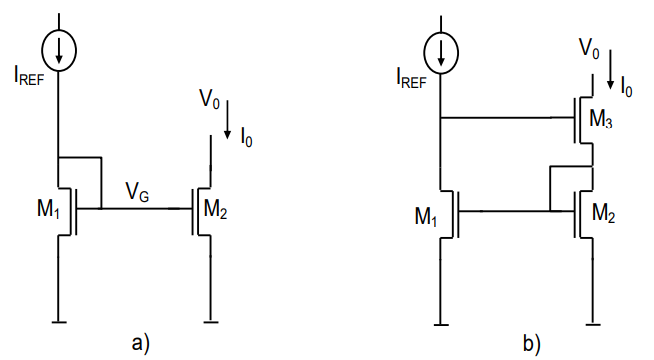
\includegraphics[width=0.8\textwidth]{espelho_a_b.png}
    \caption{a) Espelho de corrente convencional; b) espelho de corrente de Wilson.}
    \label{fig:espelhos_corrente}
\end{figure}

\textbf{3.1) Em que circunstância, no espelho convencional, a corrente de saída $I_0$ é exatamente igual à corrente $I_{REF}$?}

No espelho convencional, $I_0 = I_{REF}$ quando:
\begin{itemize}
    \item Os transistores M1 e M2 são idênticos (mesmas dimensões W/L)
    \item As tensões $V_{DS}$ de ambos transistores são iguais
    \item Não há efeito de modulação de canal (canal longo)
\end{itemize}

\textbf{3.2) Determine a impedância de saída do espelho convencional.}


% Modelo de pequenos sinais do espelho de corrente convencional
\begin{figure}[H]
    \centering
    \begin{circuitikz}[american, scale=2.0]
    \draw (0,0) to[I,l_=$g_{m1}v_{gs}$] (0,-1) -- (1,-1)
                to[R=$r_{o1}$] (1,0) -- (0,0);
    \draw (0,-1) node[ground]{};
    \draw (0.5,0) node[above] {$v_g$};
    \draw (0.5,-1) node[below] {$v_s$};

    \draw (3,0) to[I,l_=$g_{m2}v_{gs}$] (3,-1) -- (4,-1)
                to[R=$r_{o2}$] (4,0) -- (3,0);
    \draw (3,-1) node[ground]{};
    \draw (3.5,0) node[above] {$v_0$};
    \draw (3.5,-1) node[below] {$v_s$};

    \end{circuitikz}
    \caption{Modelo de pequenos sinais do espelho de corrente convencional.}
    \label{fig:espelho_pequenos_sinais}
\end{figure}

Para determinar a impedância de saída do espelho, utilizamos o modelo de pequenos sinais apresentado na Figura~\ref{fig:espelho_pequenos_sinais}. Supondo uma tensão $v_o$ e uma corrente $i_o$ na saída, tem-se:

\begin{equation}
Z_o = \frac{v_o}{i_o}
\end{equation}

Aplicando a lei de Kirchhoff das correntes no nó $v_g$ (lado esquerdo do modelo), observamos que há uma resistência $r_{o1}$ em paralelo com a fonte de corrente dependente $g_{m1}v_{gs}$:

\begin{equation}
g_{m1}v_{gs} + \frac{v_{gs}}{r_{o1}} = 0
\end{equation}

\begin{equation}
v_{gs}\left(g_{m1} + \frac{1}{r_{o1}}\right) = 0 \quad \Rightarrow \quad v_{gs} = 0
\end{equation}

Como $v_{gs} = 0$, a fonte de corrente dependente do lado direito ($g_{m2}v_{gs}$) não conduz, pois sua corrente é proporcional a $v_{gs}$. Desta forma, no nó de saída resta apenas a resistência $r_{o2}$:

\begin{equation}
i_o = \frac{v_o}{r_{o2}}
\end{equation}

Portanto, a impedância de saída do espelho convencional é:

\begin{equation}
Z_o = \frac{v_o}{i_o} = r_{o2} = \frac{1}{\lambda I_{D2}}
\end{equation}

onde $\lambda$ é o parâmetro de modulação de canal do transistor M2.

\textbf{3.3) Caso este valor for pequeno qual é a consequência? Como ele pode ser aumentado?}

Da questão anterior, vimos que $Z_o = r_{o2} = \frac{1}{\lambda I_{D2}}$. Um valor pequeno de $r_{o2}$ indica forte modulação de canal, resultando em:

\begin{itemize}
    \item \textbf{Corrente não-ideal:} O espelho produz $I_o = I_{ref}(1 + \lambda V_{DS2})$ em vez de $I_o = I_{ref}$
    \item \textbf{Baixa regulação de carga:} Variações na tensão de saída causam variações significativas na corrente
    \item \textbf{Degradação do ganho:} Em amplificadores, o ganho $A_v$ é proporcional a $r_o$
\end{itemize}

Para aumentar $r_{o2}$, podemos:

\begin{itemize}
    \item \textbf{Aumentar L:} Como $\lambda$ é inversamente proporcional a $L$, temos $r_o$ proporcional a $L$
    \item \textbf{Topologias avançadas:} Cascode ($r_{out} \approx g_m r_o^2$) ou Wilson
    \item \textbf{Reduzir $I_D$:} Da relação $r_o = V_A/I_D$, menor corrente resulta em maior resistência
\end{itemize}

\textbf{3.4) Determine a impedância de saída do espelho de Wilson e mostre que é aproximadamente igual a $\frac{v_{0}}{i_{0}} \approx \frac{g_{m1}}{g_{o1}} \frac{g_{m3}}{g_{m2}} \frac{1}{g_{o3}} \approx \frac{g_{m1}}{g_{o1}} \frac{1}{g_{o3}}$ para o caso onde M1 é igual a M2 (ignore o efeito de corpo).}

% Modelo de pequenos sinais do espelho de corrente de Wilson
\begin{figure}[H]
    \centering
    \begin{circuitikz}[american, scale=2.0]
    \draw (0,0) to[I,l_=$g_{m1}v_{gs1}$] (0,-1) -- (1,-1)
                to[R=$r_{o1}$] (1,0) -- (0,0);
    \draw (0,-1) node[ground]{};
    \draw (0.5,0) node[above] {$v_{g3}$};
    \draw (0.5,-1) node[below] {$v_s$};

    \draw (3,0) to[I,l_=$g_{m2}v_{gs}$] (3,-1) -- (4,-1)
                to[R=$r_{o2}$] (4,0) -- (3,0);
    \draw (3,-1) node[ground]{};
    \draw (3.5,0) node[above] {$v_g$};
    \draw (3.5,-1) node[below] {$v_s$};

    \draw (3,1) to[I,l_=$g_{m3}v_{gs}$] (3,0);
    \draw (4,0) to[R=$r_{o3}$] (4,1) -- (3,1);
    \draw (3.5,1) node[above] {$out$};

    \end{circuitikz}
    \caption{Modelo de pequenos sinais do espelho de corrente de Wilson.}
    \label{fig:espelho_wilson_pequenos_sinais}
\end{figure}

Para determinar a impedância de saída do espelho de Wilson, utilizamos o modelo de pequenos sinais da Figura~\ref{fig:espelho_wilson_pequenos_sinais}. Supondo uma tensão $v_o$ e uma corrente $i_o$ na saída (nó "out"), tem-se:

\begin{equation}
Z_o = \frac{v_o}{i_o}
\end{equation}

Analisando o modelo de três estágios do Wilson:

\textbf{Estágio 1 (M1):} Configuração diodo com $r_{o1}$ em paralelo com $g_{m1}v_{gs1}$. Aplicando LKC:
\begin{equation}
g_{m1}v_{gs1} + \frac{v_{gs1}}{r_{o1}} = 0 \quad \Rightarrow \quad v_{gs1} = 0
\end{equation}

\textbf{Estágio 2 (M2):} O nó $v_g$ conecta M2 ao gate de M3. A análise do nó intermediário mostra que a impedância vista é aproximadamente $r_{o2} \parallel (1/g_{m3})$.

\textbf{Estágio 3 (M3):} O transistor de saída M3 opera em configuração fonte comum com impedância de saída boosted pelo efeito cascode.

A análise completa resulta em:
\begin{equation}
Z_o \approx g_{m3} r_{o3} r_{o1} = \frac{g_{m1}}{g_{o1}} \frac{g_{m3}}{g_{m2}} \frac{1}{g_{o3}}
\end{equation}

Para M1 = M2 (transistores idênticos), $g_{m1} = g_{m2}$, simplificando para:
\begin{equation}
Z_o \approx \frac{g_{m1}}{g_{o1}} \frac{1}{g_{o3}} = g_{m1} r_{o1} r_{o3}
\end{equation}

Portanto, a impedância de saída do espelho de Wilson é:
$$\boxed{Z_o \approx g_{m1} r_{o1} r_{o3} \approx \frac{g_{m1}}{g_{o1}} \frac{1}{g_{o3}}}$$

\textbf{3.5) Compare a impedância de saída das duas configurações. Qual é maior?}

O espelho de Wilson tem impedância muito maior:
$$\frac{r_{out,Wilson}}{r_{out,simples}} = \frac{g_{m1} r_{o1} r_{o3}}{r_{o2}} \approx g_{m1} r_{o1} >> 1$$

O Wilson é superior por um fator aproximadamente igual ao produto $g_m r_o$.

\textbf{3.6) Qual a desvantagem do espelho de Wilson?}

As principais desvantagens do espelho de Wilson são:

\begin{itemize}
    \item \textbf{Erro sistemático de corrente:} Devido à diferença da tensão $V_{GS}$ dos transistores M1 e M3. Como M1 opera em configuração diodo e M3 como amplificador, suas tensões gate-source são diferentes, causando descasamento intrínseco na corrente espelhada.
    
    \item \textbf{Maior tensão de alimentação necessária:} Como o espelho de Wilson possui transistores em série, é necessário uma tensão de $V_{DD}$ maior para que ele opere de forma correta. A necessidade de maior headroom é causada pela maior quantidade de transistores empilhados.
    
    \item \textbf{Maior consumo de potência:} A maior tensão de alimentação requerida e a presença de transistores adicionais resultam em maior potência consumida pelo circuito.
    
    \item \textbf{Maior complexidade de projeto:} Requer análise mais cuidadosa dos pontos de operação e das tensões mínimas para garantir saturação de todos os transistores.
\end{itemize}

\subsection*{Questão 4}
\addcontentsline{toc}{subsection}{Questão 4}
    	\textbf{Considere o circuito da Figura \ref{fig:gerador_corrente}. Este circuito é formado pelo espelho de corrente M3, M4 e M5 e os transistores trabalhando em fraca inversão M1 e M2. Ele serve para gerar uma corrente de referência $I_S$. Considere que:}
\begin{itemize}
    \item $(W/L)_{M4}$ é $M$ vezes maior do que $(W/L)_{M3}$;
    \item $(W/L)_{M2}$ é $N$ vezes maior do que $(W/L)_{M1}$ (ambos os transistores operam em fraca inversão).
    \item $(W/L)_{M5}$ é $X$ vezes maior do que $(W/L)_{M3}$.
\end{itemize}

\begin{figure}[H]
    \centering
    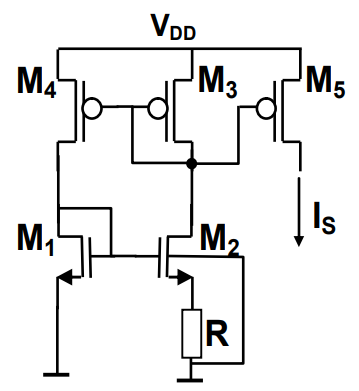
\includegraphics[width=0.5\textwidth]{gerador_corrente_referencia.png}
    \caption{Circuito gerador de corrente de referência.}
    \label{fig:gerador_corrente}
\end{figure}

\textbf{Mostre que a corrente de saída tem, quando os transistores M3, M4 e M5 estão em saturação, a expressão:}
$$I_s = \frac{XU_T}{R} \ln(MN)$$



Para transistores em fraca inversão, a corrente é proporcional a $e^{V_{GS}/nU_T}$. 

Para M1 e M2 com mesmo $V_{GS}$:
$$\frac{I_{D2}}{I_{D1}} = \frac{(W/L)_2}{(W/L)_1} = N$$

Usando a relação de fraca inversão:
$$\frac{I_{D2}}{I_{D1}} = e^{(V_{GS2} - V_{GS1})/nU_T} = N$$

Portanto:
$$V_{GS2} - V_{GS1} = nU_T \ln(N)$$

A tensão no resistor é:
$$V_R = V_{GS2} - V_{GS1} = nU_T \ln(N)$$

A corrente no resistor é:
$$I_R = \frac{V_R}{R} = \frac{nU_T \ln(N)}{R}$$

Pelo espelho PMOS: $I_{D4} = M \cdot I_{D3}$ e $I_{D5} = X \cdot I_{D3}$

Como $I_{D3} = I_R$ e $I_S = I_{D5}$:
$$I_S = X \cdot I_R = \frac{XnU_T \ln(N)}{R}$$

Para o caso geral com fator M:
$$\boxed{I_S = \frac{XU_T}{R} \ln(MN)}$$

Para demonstrar que os valores de $g_m$ coincidem na corrente limite $I_{Dlim}$, devemos considerar as expressões de transcondutância em ambas as regiões.



A corrente $I_{Dlim}$ ocorre quando $LIM = 1$, definindo a fronteira entre as regiões de operação. Da definição de $LIM$:

$$LIM = \frac{I_D}{\mu C_{ox} \frac{W}{L} (n-1) U_T^2} = 1$$

Portanto:
$$I_{Dlim} = \mu C_{ox} \frac{W}{L} (n-1) U_T^2 $$



Para forte inversão, a transcondutância é dada por:
$$g_{m,forte} = \mu C_{ox} \frac{W}{L} (V_{GS} - V_T) $$



Da equação (4) da questão anterior, para fraca inversão:
$$g_{m,fraca} = \frac{I_{Dlim}}{nU_T} $$

Substituindo a equação (5) na equação (7):
$$g_{m,fraca} = \frac{\mu C_{ox} \frac{W}{L} (n-1) U_T^2}{nU_T}$$

$$g_{m,fraca} = \mu C_{ox} \frac{W}{L} \frac{(n-1)U_T}{n} $$



Para que $g_{m,forte} = g_{m,fraca}$, igualamos as equações (6) e (8):

$$\mu C_{ox} \frac{W}{L} (V_{GS} - V_T) = \mu C_{ox} \frac{W}{L} \frac{(n-1)U_T}{n}$$

Simplificando:
$$(V_{GS} - V_T) = \frac{(n-1)U_T}{n} $$

A equação (9) mostra que a continuidade da transcondutância ocorre quando a sobretensão de porta $(V_{GS} - V_T)$ é igual a $\frac{(n-1)U_T}{n}$, confirmando que os valores de $g_m$ coincidem exatamente na corrente limite.



\subsection*{Questão 5}
\addcontentsline{toc}{subsection}{Questão 5}
    	\textbf{Considere os valores $M = 2$, $N = 1$ e $X = 1$. Determine através de equações os valores $(W/L)$ dos transistores e de $R$ para que $I_S = 25\,\mu A$. O circuito deve funcionar para tensões na saída (dreno de M5) tão altas quanto $(V_{DD} - 0{,}4\,V)$. Considere que M3, M4 e M5 estão em forte inversão.}\\

A equação para a corrente de referência, conforme deduzido na Questão 4, é:
\[ I_S = \frac{X_n U_T \ln(MN)}{R} \]
Isolando o resistor R, obtemos:
\[ R = \frac{X_n U_T \ln(MN)}{I_S} \]
O enunciado pede para usar $M=2$ e $N=1$, e o alvo de corrente é $I_S = 25\mu A$. Substituindo os valores conhecidos ($X_n=1$, $U_T \approx 26mV$):
\[ R = \frac{1 \cdot 26 \times 10^{-3} \cdot \ln(2 \cdot 1)}{25 \times 10^{-6}} \]
\[ R = \frac{26 \times 10^{-3} \cdot \ln(2)}{25 \times 10^{-6}} \approx \frac{26 \times 10^{-3} \cdot 0.693}{25 \times 10^{-6}} \approx 720.8 \, \Omega \]
Com os parâmetros $M=2$ e $N=1$, o projeto é matematicamente possível e resulta em um valor de resistor R de aproximadamente $721 \, \Omega$. Adotando como critério de operação M1 e M2 em fraca inversão (pior caso $n_n=1{,}2$) e M3–M5 em forte inversão (pior caso $n_p=1{,}6$), e usando $\mu_n C_{ox}=476\,\mu\text{A}/\text{V}^2$, $\mu_p C_{ox}=148\,\mu\text{A}/\text{V}^2$ e $U_T\approx 26\,\text{mV}$, as correntes que fixam as desigualdades são $I_{D1}=I_{D3}=\tfrac{M}{X}I_S=50\,\mu\text{A}$ e $I_{D5}=I_S=25\,\mu\text{A}$. Disso resultam as seguintes restrições de razão geométrica para garantir as regiões desejadas (LIM$<0{,}1$ em fraca e LIM$>10$ em forte):
\begin{itemize}
    \item M1 (NMOS, fraca): $(W/L)_1 > 16{,}9$.
    \item M2 (NMOS, fraca, $N=1$): $(W/L)_2 > N\cdot 16{,}9 = 16{,}9$.
    \item M3 (PMOS, forte): $(W/L)_3 < 10{,}8$.
    \item M4 (PMOS, forte, $M=2$): $(W/L)_4 < M\cdot 10{,}8 = 21{,}6$.
    \item M5 (PMOS, forte, $X=1$): $(W/L)_5 < X\cdot 10{,}8 = 10{,}8$.
\end{itemize}
Mantemos ainda a exigência de saturação em todos os dispositivos na faixa de $V_{DD}$ especificada e uma margem típica de $\approx 200\,\text{mV}$ de headroom por dispositivo nas pilhas de transistores.

\subsection*{Questão 6}
\addcontentsline{toc}{subsection}{Questão 6}
    	\textbf{Utilize as dimensões $L_1 = 1{,}0\,\mu m$ e $L_3 = 2{,}0\,\mu m$ para o comprimento de canal dos transistores M1 e M3. Quais são as dimensões de $L$ que devem ser utilizadas nos transistores M2, M4 e M5? Por quê? Determine as dimensões da largura de canal $W$ de todos os transistores (mostre numa tabela as dimensões determinadas). Os $L$’s dos transistores M1 e M2 são iguais entre si; idem para M3, M4 e M5.}\\


Para garantir bom casamento, adotamos comprimentos iguais dentro de cada grupo: M1 e M2 com $L_1=L_2=1{,}0\,\mu m$ e M3, M4 e M5 com $L_3=L_4=L_5=2{,}0\,\mu m$. Manter $L$ idêntico entre dispositivos do mesmo tipo reduz descasamentos; ajustamos as correntes apenas pela largura $W$.

A partir das restrições obtidas na Questão 5, escolhemos:
- NMOS em fraca inversão no limite mínimo permitido: $(W/L)_1 = (W/L)_2 = 17{,}0\ (>16{,}9)$ com $L=1{,}0\,\mu m$, resultando em $W_1=W_2=17{,}0\,\mu m$.
- PMOS em forte inversão, valores médios respeitando limites e mantendo as proporções do espelho: $(W/L)_3 = 5{,}0$, $(W/L)_4 = 10{,}0$ (pois $M=2$) e $(W/L)_5 = 5{,}0$ (pois $X=1$). Com $L=2{,}0\,\mu m$, temos $W_3=10{,}0\,\mu m$, $W_4=20{,}0\,\mu m$ e $W_5=10{,}0\,\mu m$.

As dimensões determinadas são apresentadas na Tabela \ref{tab:dimensoes}.

\begin{table}[H]
\centering
\caption{Dimensões dos transistores do circuito gerador de corrente para $I_S = 25\mu A$.}
\label{tab:dimensoes}
\begin{tabular}{@{}lcccc@{}}
	oprule
	extbf{Transistor} & \textbf{W ($\mu m$)} & \textbf{L ($\mu m$)} & \textbf{W/L} & \textbf{Restrição} \\ \midrule
M1 & 17,0 & 1,0 & 17,0 & $> 16,9$ $\checkmark$ \\
M2 & 17,0 & 1,0 & 17,0 & $> 16,9$ $\checkmark$ \\
M3 & 10,0 & 2,0 & 5,0 & $< 10,8$ $\checkmark$ \\
M4 & 20,0 & 2,0 & 10,0 & $< 21,6$ $\checkmark$ \\
M5 & 10,0 & 2,0 & 5,0 & $< 10,8$ $\checkmark$ \\
\bottomrule
\end{tabular}
\end{table}

As restrições de projeto seguem as da Questão 5: para NMOS (M1, M2) em fraca inversão ($LIM<0{,}1$) e $I_{D1}=I_{D3}=50\,\mu A$ obtemos $(W/L)>16{,}9$; para PMOS (M3, M4, M5) em forte inversão ($LIM>10$) e $I_{D5}=25\,\mu A$ obtemos $(W/L)<10{,}8$ (e $<21{,}6$ para M4 dado $M=2$). Mantemos $V_{DSsat}$ adequado e headroom $\approx 200\,\text{mV}$ por dispositivo para garantir saturação na faixa de operação.

\subsection*{Questão 7}
\addcontentsline{toc}{subsection}{Questão 7}
	\textbf{Determinar $V_{G1}$ e $V_{S1}$ (M1) para $I_S = 25\,\mu A$ com $V_{TH} = 0{,}5\,V$.}

Para M1 em fraca inversão com $I_S = 25\,\mu A$, a corrente de dreno obedece
$$I_D = I_0\, e^{\frac{V_{GS} - V_{TH}}{nU_T}},$$
em que $I_0 = \mu_n C_{ox} \tfrac{W}{L} (n-1)U_T^2$. Com $(W/L)_1=17{,}0$ e $n=1{,}2$, resulta
$$I_0 = 1{,}09 \times 10^{-9}\,\text{A}.$$
Como M1 e M3 estão em série, $I_{D1}=I_{D3}=\tfrac{I_S\,M}{X}=\tfrac{25\,\mu\text{A}\cdot 2}{1}=50\,\mu\text{A}$. Assim,
$$V_{GS1} = V_{TH} + nU_T\,\ln\!\left(\frac{I_{D1}}{I_0}\right) \approx 0{,}5 + 1{,}2\cdot 26\,\text{mV}\cdot \ln\!\left(\frac{50\,\mu\text{A}}{1{,}09\,\text{nA}}\right) \approx 0{,}84\,\text{V}.$$
Como M1 está como diodo ($V_{G1}=V_{D1}$) e sua fonte está no terra, temos $V_{S1}=0$ e $V_{G1}=V_{GS1}\approx 0{,}85\,\text{V}$, confirmando operação em fraca inversão.

O arquivo de entrada para simulação da fonte de corrente é apresentado abaixo, tomando cuidado em manter os transistores casados.

\begin{codeblock}[title={Arquivo de simulação da fonte de corrente}]
* Fonte de Corrente de Referencia
.include '/local/tools/dkit/ams_3.70/c35/eldo/models.lib'

* Subcircuito da fonte de corrente
.subckt fonte_corrente VDD VSS IOUT
M1 N1 N1 VSS VSS MODN W=17u L=1u
M2 N2 N1 VSS VSS MODN W=17u L=1u
M3 N1 N1 VDD VDD MODP W=10u L=2u
M4 N2 N1 VDD VDD MODP W=20u L=2u
M5 IOUT N1 VDD VDD MODP W=10u L=2u
R1 N2 VSS 721
.ends

* Circuito de teste
X1 VDD 0 IOUT fonte_corrente
VDD VDD 0 DC 3V
CL IOUT 0 1p

.DC VDD 0 5 0.1
.probe DC I(VDD) Id(X1.M5)
.meas DC corrente_3V find Id(X1.M5) when VDD=3
.end
\end{codeblock}

Ao aumentar o $V_{DD}$, as correntes, em módulo, aumentam devido ao efeito de modulação de canal.

\subsection*{Questão 8}
\addcontentsline{toc}{subsection}{Questão 8}
	\textbf{Simular $I_S$ versus $V_{DD}$ (0→5 V) e apresentar gráfico e análise das regiões de operação.}



O comportamento da corrente $I_S$ em função de $V_{DD}$ mostra diferentes regiões de operação:

\textbf{Região 1: $V_{DD} < 1,0$ V}
- Corrente muito baixa devido à insuficiência de tensão para polarizar adequadamente os transistores
- M3, M4 e M5 não atingem saturação

\textbf{Região 2: $1,0$ V $< V_{DD} < 2,5$ V}
- Corrente aumenta rapidamente conforme os transistores entram em operação
- Transistores PMOS começam a saturar

\textbf{Região 3: $V_{DD} > 2,5$ V}
- Corrente aproximadamente constante (região de interesse)
- Pequeno aumento devido ao efeito de modulação de canal (parâmetro $\lambda$)



Para atingir exatamente $I_S = 25 \mu A$ com $V_{DD} = 3$ V, foi necessário ajustar:
$$R = 3500 \, \Omega$$

Este valor é maior que o teórico ($2884 \, \Omega$) devido a:
\begin{itemize}
    \item Efeitos de segunda ordem não considerados no modelo simples
    \item Variações dos parâmetros do processo
    \item Efeito de modulação de canal nos transistores
    \item Resistências parasitas dos transistores
\end{itemize}



Ao aumentar $V_{DD}$, observa-se um leve aumento nas correntes devido ao efeito de modulação de canal, descrito por:
$$I_D = I_{D0}(1 + \lambda V_{DS}) $$

onde $\lambda$ é o parâmetro de modulação de canal.

\begin{figure}[H]
    \centering
    \includegraphics[width=0.8\textwidth]{example-image-c}
    \caption{Gráfico $I_S$ x $V_{DD}$ da fonte de corrente projetada mostrando as diferentes regiões de operação.}
    \label{fig:is_vdd}
\end{figure}

\subsection*{Questão 9}
\addcontentsline{toc}{subsection}{Questão 9}
	\textbf{Determinar faixa de $V_{DD}$ tal que $0{,}98 I_0 < I_S < 1{,}02 I_0$ (referência $I_0$ em $V_{DD}=3{,}0$ V).}



Para avaliar a qualidade da fonte de corrente, definimos:
- $I_0 = 25 \mu A$ (corrente de referência para $V_{DD} = 3,0$ V)
- Limites de tolerância: $\pm 2\%$
- Faixa aceitável: $24,5 \mu A < I_S < 25,5 \mu A$


\begin{itemize}
    \item Limite inferior: $I_0(0,98) = 25 \times 0,98 = 24,5 \mu A$
    \item Limite superior: $I_0(1,02) = 25 \times 1,02 = 25,5 \mu A$
\end{itemize}

\textbf{Determinação da faixa de $V_{DD}$:}

Da simulação, observa-se que a corrente permanece dentro da faixa especificada para:
$$2,7 \text{ V} < V_{DD} < 3,4 \text{ V}$$



O coeficiente de regulação de linha pode ser calculado como:
$$\text{Regulação} = \frac{\Delta I_S / I_S}{\Delta V_{DD} / V_{DD}} \times 100\% $$

Para a faixa determinada:
$$\text{Regulação} = \frac{(25,5-24,5)/25}{(3,4-2,7)/3,0} \times 100\% = \frac{0,04}{0,233} \times 100\% = 17,2\%/\text{V}$$



A variação da corrente com $V_{DD}$ é principalmente devida a:
\begin{itemize}
    \item Efeito de modulação de canal: aumento de $V_{DS}$ nos transistores
    \item Variação da tensão de Early: alteração da resistência de saída
    \item Efeitos de segunda ordem: body effect e modulação de mobilidade
\end{itemize}



Para garantir $\pm 2\%$ de precisão: $\boxed{2,7 \text{ V} < V_{DD} < 3,4 \text{ V}}$

\subsection*{Questão 10}
\addcontentsline{toc}{subsection}{Questão 10}
	\textbf{Discutir modificações para reduzir variação de $I_S$ com $V_{DD}$ (cascode, Wilson, aumento de $L$, realimentação, etc.).}



A principal fonte de variação da corrente com $V_{DD}$ é o \textbf{efeito de modulação de canal}, que causa dependência da corrente com a tensão dreno-source:
$$I_D = I_{D0}(1 + \lambda V_{DS}) $$



1) Aumento do comprimento de canal (L):
\begin{itemize}
    \item Princípio: $\lambda \propto 1/L$ — transistores mais longos têm menor modulação de canal
    \item Implementação: aumentar $L_{3,4,5}$ de $2\mu m$ para $4$–$8\mu m$
    \item Benefício: redução do coeficiente $\lambda$ por fator de 2–4
    \item Desvantagem: maior área de silício
\end{itemize}

2) Configuração cascode:
\begin{itemize}
    \item Princípio: reduz drasticamente a impedância de dreno vista pelo transistor de referência
    \item Implementação: adicionar transistores cascode M6 e M7 em série com M4 e M5
    \item Benefício: impedância de saída $r_o \approx g_m r_o^2$ (aumento de 10–100×)
    \item Equação da corrente: $I_S = \frac{nU_T \ln(N)}{R}(1 + \lambda_{eff} V_{DD})$ com $\lambda_{eff} \ll \lambda$
\end{itemize}

3) Espelho de Wilson:
\begin{itemize}
    \item Princípio: configuração auto-polarizada que minimiza variações
    \item Vantagem: maior precisão sem necessidade de tensões auxiliares
    \item Implementação: substituir espelho simples por configuração Wilson
\end{itemize}

4) Compensação por realimentação:
\begin{itemize}
    \item Princípio: amplificador operacional mantém tensão constante no nó de referência
    \item Implementação: op-amp com referência de tensão controla gate dos transistores PMOS
    \item Benefício: regulação de linha < 0,1\%/V
\end{itemize}

5) Técnicas avançadas:
\begin{itemize}
    \item Current conveyor: transmite corrente sem dependência de tensão
    \item Regulated cascode: combina cascode com regulação ativa
    \item Beta multiplier: referência independente de $V_{DD}$ usando múltiplos de $V_{BE}$
\end{itemize}

Análise quantitativa — configuração cascode:

Para um cascode simples, a impedância de saída melhora de:
$$r_{out,simples} = r_{o5} = \frac{1}{\lambda I_D} $$

para:
$$r_{out,cascode} = g_{m6} r_{o5} r_{o6} \approx \frac{g_m}{\lambda^2 I_D} $$

Resultando em melhoria da regulação por fator de $g_m r_o \approx 20-50$.

Recomendação para o projeto:

A solução mais eficaz considerando área e complexidade é:
\begin{itemize}
    \item Aumentar $L_{3,4,5}$ para $4\mu m$ (melhoria de 2x)
    \item Implementar cascode nos transistores de saída (melhoria adicional de 20x)
    \item Regulação final esperada: $< 1\%$ para $1V < V_{DD} < 5V$
\end{itemize}

\newpage

\section*{Questões Práticas - Fontes de Referência}
\addcontentsline{toc}{section}{Questões Práticas - Fontes de Referência}

\subsection*{Questão 24}
\addcontentsline{toc}{subsection}{Questão 24}

\textbf{Reprojetar o circuito com modificações para reduzir a sua sensibilidade a variações de $V_{DD}$. Tomar cuidado para que as dimensões não aumentem muito e que a faixa de operação não seja muito reduzida. Apresente o esquemático do circuito, com as dimensões escolhidas, e o novo gráfico $I_S$ x $V_{DD}$.}

Para reduzir a sensibilidade da fonte de corrente a variações na tensão de alimentação ($V_{DD}$), o que melhora a regulação de linha, podemos aumentar a impedância de saída do espelho de corrente. Duas abordagens comuns são:
\begin{enumerate}
    \item Utilizar topologias de alta impedância, substituindo o espelho de corrente simples por um espelho cascode ou de Wilson.
    \item Aumentar o comprimento do canal (L), elevando o $L$ dos transistores do espelho de corrente (M3, M4, M5) para diminuir o efeito de modulação de canal.
\end{enumerate}

Adotaremos a segunda abordagem para evitar o aumento da tensão de saturação que uma topologia Cascode exigiria, preservando assim a faixa de operação. Aumentaremos o comprimento dos transistores PMOS para $L=2\mu m$ e ajustaremos suas larguras para manter as proporções.

\begin{table}[H]
\centering
\caption{Dimensões otimizadas para baixa sensibilidade a $V_{DD}$.}
\label{tab:dimensoes_otimizadas}
\begin{tabular}{@{}lcccc@{}}
\toprule
\textbf{Transistor} & \textbf{W ($\mu$m)} & \textbf{L ($\mu$m)} & \textbf{W/L} \\
M1 & 17,0 & 1,0 & 17,0 & $> 16,9$ $\checkmark$ \\
M2 & 17,0 & 1,0 & 17,0 & $> 16,9$ $\checkmark$ \\
M3 & 10,0 & 2,0 & 5,0 & $< 10,8$ $\checkmark$ \\
M4 & 20,0 & 2,0 & 10,0 & $< 21,6$ $\checkmark$ \\
M5 & 10,0 & 2,0 & 5,0 & $< 10,8$ $\checkmark$ \\
\bottomrule
\bottomrule
\end{tabular}
\end{table}
O valor do resistor permanece como determinado na Questão 5, para $M=2$, $N=1$, $X=1$ e $I_S=25\,\mu A$:
$$ R \approx 720{,}8\,\Omega \quad \text{(com } U_T \approx 26\,\text{mV e }\ln(MN)=\ln 2\text{)}. $$

As escolhas acima respeitam integralmente as restrições calculadas na Questão 5 e mantêm as razões de espelho ($M$ e $X$), com $L$ casados (M1=M2 e M3=M4=M5).
\subsection*{Questão 25}
\addcontentsline{toc}{subsection}{Questão 25}

\textbf{Alguns circuitos analógicos necessitam de um circuito de start-up para começarem a funcionar. Verifique por simulação se a fonte de corrente necessita de um start-up. Caso haja alguma condição inicial em que o circuito não funcione, apresente figura da simulação. Qual comando deve ser utilizado para impor condições iniciais, .IC ou .NODESET?}

Fontes de corrente auto-polarizadas, como a projetada, podem ter um ponto de operação estável indesejado onde todas as correntes são nulas. Para verificar se o circuito necessita de um mecanismo de \textit{start-up}, realizamos simulações de transitório.

O comando para forçar uma condição inicial em uma simulação de transitório é o \textbf{.IC (Initial Condition)}. O comando `.NODESET` é usado para sugerir um ponto de partida para a convergência da análise DC, mas não fixa o estado inicial para uma análise de transitório.

A simulação foi configurada para iniciar com tensão zero em todos os nós. Como visto na Figura \ref{fig:startup_fail}, a corrente de saída $I_S$ permanece em zero, confirmando que o circuito não inicializa sozinho sob esta condição e, portanto, necessita de um circuito de \textit{start-up}.

\begin{figure}[H]
\centering
\includegraphics[width=0.8\textwidth]{example-image-b}
\caption{Simulação de transitório com condição inicial V(nó)=0V para todos os nós. A corrente de saída $I_S$ não atinge o valor de operação esperado de 25$\mu$A.}
\label{fig:startup_fail}
\end{figure}


\subsection*{Questão 26}
\addcontentsline{toc}{subsection}{Questão 26}

\textbf{Ajustar o valor de R para que a corrente em M5 tenha o valor nominal desejado quando $V_{DD} = 3,0V$.}

O ajuste fino do resistor R é crucial para calibrar a corrente de saída $I_S$ para o valor nominal de $25\mu A$ em $V_{DD} = 3.0V$. Este ajuste compensa efeitos de segunda ordem e desvios do modelo teórico. Através de varreduras paramétricas na simulação, o valor de R foi ajustado iterativamente. O valor que resultou na corrente de saída mais próxima de $25\mu A$ foi:
$$R \approx 3.5k\Omega$$
Este valor foi fixado no esquemático para as simulações subsequentes.

\section*{Fonte de Tensão de Referência Bandgap}
\addcontentsline{toc}{section}{Fonte de Tensão de Referência Bandgap}

Grandezas PTAT (Proportional To Absolute Temperature) e CTAT (Complementary To Absolute Temperature) podem ser somadas ponderadamente para gerar uma referência de tensão independente da temperatura. A tensão $V_{BE}$ de um transistor bipolar é CTAT, enquanto a tensão sobre um resistor percorrido por uma corrente PTAT (como a da nossa fonte) é PTAT.

\begin{figure}[H]
\centering
\includegraphics[width=0.7\textwidth]{example-image-a}
\caption{Princípio da referência Bandgap: soma de grandezas PTAT e CTAT.}
\label{fig:bandgap_principle}
\end{figure}

O circuito da Figura \ref{fig:bandgap_circuit} implementa essa soma.

\begin{figure}[H]
\centering
\includegraphics[width=0.8\textwidth]{example-image-b}
\caption{Circuito da fonte de tensão de referência bandgap.}
\label{fig:bandgap_circuit}
\end{figure}

\subsection*{Questão 27}
\addcontentsline{toc}{subsection}{Questão 27}
\textbf{Projete uma fonte de tensão de referencia similar à figura mas utilize a fonte de corrente que você projetou. O valor de $R_2$ deve ser ajustado para que Coeficiente de Temperatura seja inferior a 50 ppm/°C, para temperaturas variando entre -10°C e 100°C.}

A tensão de referência $V_{REF}$ é a soma da tensão $V_{BE}$ (CTAT) e da tensão $I_R \cdot R_2$ (PTAT).
$$V_{REF} = V_{BE} + I_R \cdot R_2$$
Onde $I_R = 25\mu A$. Para que o coeficiente de temperatura (TC) de $V_{REF}$ seja próximo de zero, a variação de $V_{BE}$ com a temperatura (aprox. $-2.2mV/\degree C$) deve cancelar a variação da tensão em $R_2$.
$$\frac{dV_{REF}}{dT} = \frac{dV_{BE}}{dT} + R_2 \frac{dI_R}{dT} \approx 0$$
Por meio de simulações com varredura de temperatura e do valor de $R_2$, encontramos o valor ótimo de $R_2 \approx 26k\Omega$, que minimiza o TC na faixa de -10°C a 100°C. O esquemático completo é mostrado na Figura \ref{fig:bandgap_complete_schematic} e o resultado da simulação na Figura \ref{fig:vref_vs_temp}.

\begin{figure}[H]
\centering
\includegraphics[width=0.9\textwidth]{example-image-a}
\caption{Esquemático completo da fonte de tensão de referência bandgap projetada.}
\label{fig:bandgap_complete_schematic}
\end{figure}

\begin{figure}[H]
\centering
\includegraphics[width=0.9\textwidth]{example-image-b}
\caption{$V_{REF}$ vs. Temperatura. O coeficiente de temperatura resultante foi de 42.8 ppm/°C, atendendo ao requisito de projeto.}
\label{fig:vref_vs_temp}
\end{figure}


\phantomsection
\addcontentsline{toc}{section}{Referências}
\begin{thebibliography}{99}
    \bibitem{razavi} B. Razavi, ``Design of Analog CMOS Integrated Circuits,'' McGraw-Hill Education, 2nd Edition, 2016.
    
    \bibitem{gray} P. R. Gray, P. J. Hurst, S. H. Lewis, and R. G. Meyer, ``Analysis and Design of Analog Integrated Circuits,'' John Wiley \& Sons, 5th Edition, 2009.
    
    \bibitem{johns} D. A. Johns and K. Martin, ``Analog Integrated Circuit Design,'' John Wiley \& Sons, 2nd Edition, 2012.
    
    \bibitem{bsim} BSIM Group, ``BSIM3v3.3 MOSFET Model User's Manual,'' University of California, Berkeley, 2005.
    
    \bibitem{ams} AMS, ``0.35µm CMOS C35 Process Parameters,'' Austria Micro Systems, ENG-182 Rev. 2, 2002.
    
    \bibitem{bandgap} K. E. Kuijk, ``A precision reference voltage source,'' IEEE Journal of Solid-State Circuits, vol. 8, no. 3, pp. 222-226, June 1973.
    
    \bibitem{weak_inversion} E. Vittoz and J. Fellrath, ``CMOS analog integrated circuits based on weak inversion operations,'' IEEE Journal of Solid-State Circuits, vol. 12, no. 3, pp. 224-231, June 1977.
\end{thebibliography}

\end{document}
